%%%%%%%%%%%%%%%%%%%%%%%%%%%%%%%%%%%%%%%%%%%%%%%%%%%%%%%%%%%%%%%
%
% Welcome to Overleaf --- just edit your LaTeX on the left,
% and we'll compile it for you on the right. If you open the
% 'Share' menu, you can invite other users to edit at the same
% time. See www.overleaf.com/learn for more info. Enjoy!
%
%%%%%%%%%%%%%%%%%%%%%%%%%%%%%%%%%%%%%%%%%%%%%%%%%%%%%%%%%%%%%%%
% \documentclass is a command

\documentclass[12pt, letterpaper]{article}
\usepackage{geometry}
% graphicx package allows images to be embedded in a document
\usepackage{graphicx}
\title{Sample LaTex Document}
\author{Simon Fermor\thanks{with help from Arthur}}
\date{December 2022}
\begin{document}
\maketitle
\tableofcontents

\section{Headings are numbered}
\subsection{sub-headings are also numbered}
% \textbf is the command for bold font
% \textid is the command for italicized text
% \underline is the command for underline
% \emph allows text to be emphasized depending on context
\textbf{This} is the second \textit{paragraph}
First document created in \LaTeX. This is a simple example, with no extra parameters or packages included.
See below for figure \ref{fig:rochester}, on page \pageref{fig:rochester}
% The itemize tag is used to create bullets
% The begin / end tags create an environment
\begin{itemize}
\item test
\item another test
\end{itemize}
% when importing graphics avoid spaces and multiple ... and use lower case for filename extensions
\begin{figure}[ht]
\centering
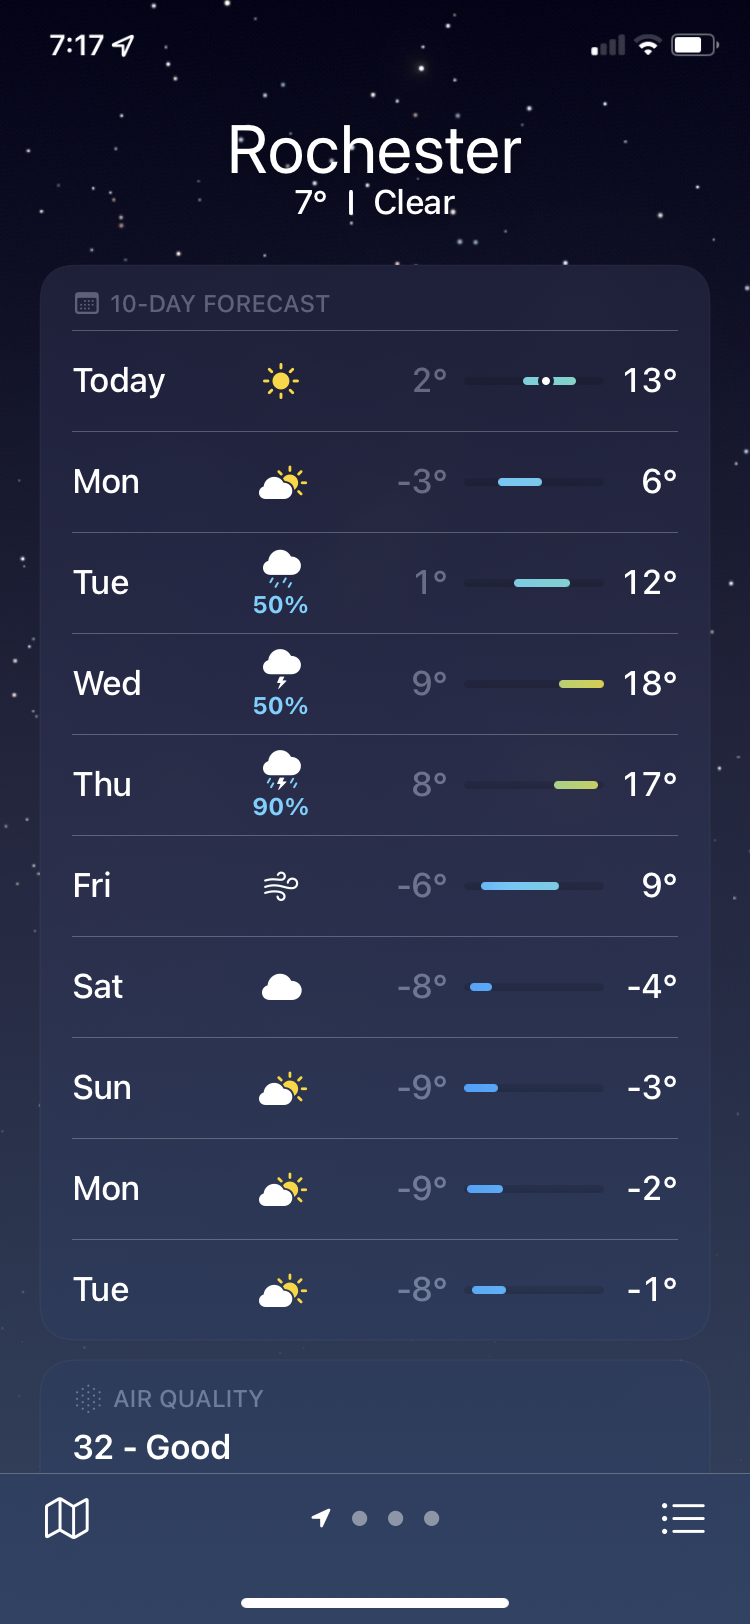
\includegraphics[width=0.5\textwidth]{20221107_011741000_iOS.png}
\caption{Nice weather}
\label{fig:rochester}
\end{figure}
\end{document}